% Options for packages loaded elsewhere
% Options for packages loaded elsewhere
\PassOptionsToPackage{unicode}{hyperref}
\PassOptionsToPackage{hyphens}{url}
\PassOptionsToPackage{dvipsnames,svgnames,x11names}{xcolor}
%
\documentclass[
  letterpaper,
  DIV=11,
  numbers=noendperiod]{scrartcl}
\usepackage{xcolor}
\usepackage{amsmath,amssymb}
\setcounter{secnumdepth}{-\maxdimen} % remove section numbering
\usepackage{iftex}
\ifPDFTeX
  \usepackage[T1]{fontenc}
  \usepackage[utf8]{inputenc}
  \usepackage{textcomp} % provide euro and other symbols
\else % if luatex or xetex
  \usepackage{unicode-math} % this also loads fontspec
  \defaultfontfeatures{Scale=MatchLowercase}
  \defaultfontfeatures[\rmfamily]{Ligatures=TeX,Scale=1}
\fi
\usepackage{lmodern}
\ifPDFTeX\else
  % xetex/luatex font selection
\fi
% Use upquote if available, for straight quotes in verbatim environments
\IfFileExists{upquote.sty}{\usepackage{upquote}}{}
\IfFileExists{microtype.sty}{% use microtype if available
  \usepackage[]{microtype}
  \UseMicrotypeSet[protrusion]{basicmath} % disable protrusion for tt fonts
}{}
\makeatletter
\@ifundefined{KOMAClassName}{% if non-KOMA class
  \IfFileExists{parskip.sty}{%
    \usepackage{parskip}
  }{% else
    \setlength{\parindent}{0pt}
    \setlength{\parskip}{6pt plus 2pt minus 1pt}}
}{% if KOMA class
  \KOMAoptions{parskip=half}}
\makeatother
% Make \paragraph and \subparagraph free-standing
\makeatletter
\ifx\paragraph\undefined\else
  \let\oldparagraph\paragraph
  \renewcommand{\paragraph}{
    \@ifstar
      \xxxParagraphStar
      \xxxParagraphNoStar
  }
  \newcommand{\xxxParagraphStar}[1]{\oldparagraph*{#1}\mbox{}}
  \newcommand{\xxxParagraphNoStar}[1]{\oldparagraph{#1}\mbox{}}
\fi
\ifx\subparagraph\undefined\else
  \let\oldsubparagraph\subparagraph
  \renewcommand{\subparagraph}{
    \@ifstar
      \xxxSubParagraphStar
      \xxxSubParagraphNoStar
  }
  \newcommand{\xxxSubParagraphStar}[1]{\oldsubparagraph*{#1}\mbox{}}
  \newcommand{\xxxSubParagraphNoStar}[1]{\oldsubparagraph{#1}\mbox{}}
\fi
\makeatother

\usepackage{color}
\usepackage{fancyvrb}
\newcommand{\VerbBar}{|}
\newcommand{\VERB}{\Verb[commandchars=\\\{\}]}
\DefineVerbatimEnvironment{Highlighting}{Verbatim}{commandchars=\\\{\}}
% Add ',fontsize=\small' for more characters per line
\usepackage{framed}
\definecolor{shadecolor}{RGB}{241,243,245}
\newenvironment{Shaded}{\begin{snugshade}}{\end{snugshade}}
\newcommand{\AlertTok}[1]{\textcolor[rgb]{0.68,0.00,0.00}{#1}}
\newcommand{\AnnotationTok}[1]{\textcolor[rgb]{0.37,0.37,0.37}{#1}}
\newcommand{\AttributeTok}[1]{\textcolor[rgb]{0.40,0.45,0.13}{#1}}
\newcommand{\BaseNTok}[1]{\textcolor[rgb]{0.68,0.00,0.00}{#1}}
\newcommand{\BuiltInTok}[1]{\textcolor[rgb]{0.00,0.23,0.31}{#1}}
\newcommand{\CharTok}[1]{\textcolor[rgb]{0.13,0.47,0.30}{#1}}
\newcommand{\CommentTok}[1]{\textcolor[rgb]{0.37,0.37,0.37}{#1}}
\newcommand{\CommentVarTok}[1]{\textcolor[rgb]{0.37,0.37,0.37}{\textit{#1}}}
\newcommand{\ConstantTok}[1]{\textcolor[rgb]{0.56,0.35,0.01}{#1}}
\newcommand{\ControlFlowTok}[1]{\textcolor[rgb]{0.00,0.23,0.31}{\textbf{#1}}}
\newcommand{\DataTypeTok}[1]{\textcolor[rgb]{0.68,0.00,0.00}{#1}}
\newcommand{\DecValTok}[1]{\textcolor[rgb]{0.68,0.00,0.00}{#1}}
\newcommand{\DocumentationTok}[1]{\textcolor[rgb]{0.37,0.37,0.37}{\textit{#1}}}
\newcommand{\ErrorTok}[1]{\textcolor[rgb]{0.68,0.00,0.00}{#1}}
\newcommand{\ExtensionTok}[1]{\textcolor[rgb]{0.00,0.23,0.31}{#1}}
\newcommand{\FloatTok}[1]{\textcolor[rgb]{0.68,0.00,0.00}{#1}}
\newcommand{\FunctionTok}[1]{\textcolor[rgb]{0.28,0.35,0.67}{#1}}
\newcommand{\ImportTok}[1]{\textcolor[rgb]{0.00,0.46,0.62}{#1}}
\newcommand{\InformationTok}[1]{\textcolor[rgb]{0.37,0.37,0.37}{#1}}
\newcommand{\KeywordTok}[1]{\textcolor[rgb]{0.00,0.23,0.31}{\textbf{#1}}}
\newcommand{\NormalTok}[1]{\textcolor[rgb]{0.00,0.23,0.31}{#1}}
\newcommand{\OperatorTok}[1]{\textcolor[rgb]{0.37,0.37,0.37}{#1}}
\newcommand{\OtherTok}[1]{\textcolor[rgb]{0.00,0.23,0.31}{#1}}
\newcommand{\PreprocessorTok}[1]{\textcolor[rgb]{0.68,0.00,0.00}{#1}}
\newcommand{\RegionMarkerTok}[1]{\textcolor[rgb]{0.00,0.23,0.31}{#1}}
\newcommand{\SpecialCharTok}[1]{\textcolor[rgb]{0.37,0.37,0.37}{#1}}
\newcommand{\SpecialStringTok}[1]{\textcolor[rgb]{0.13,0.47,0.30}{#1}}
\newcommand{\StringTok}[1]{\textcolor[rgb]{0.13,0.47,0.30}{#1}}
\newcommand{\VariableTok}[1]{\textcolor[rgb]{0.07,0.07,0.07}{#1}}
\newcommand{\VerbatimStringTok}[1]{\textcolor[rgb]{0.13,0.47,0.30}{#1}}
\newcommand{\WarningTok}[1]{\textcolor[rgb]{0.37,0.37,0.37}{\textit{#1}}}

\usepackage{longtable,booktabs,array}
\usepackage{calc} % for calculating minipage widths
% Correct order of tables after \paragraph or \subparagraph
\usepackage{etoolbox}
\makeatletter
\patchcmd\longtable{\par}{\if@noskipsec\mbox{}\fi\par}{}{}
\makeatother
% Allow footnotes in longtable head/foot
\IfFileExists{footnotehyper.sty}{\usepackage{footnotehyper}}{\usepackage{footnote}}
\makesavenoteenv{longtable}
\usepackage{graphicx}
\makeatletter
\newsavebox\pandoc@box
\newcommand*\pandocbounded[1]{% scales image to fit in text height/width
  \sbox\pandoc@box{#1}%
  \Gscale@div\@tempa{\textheight}{\dimexpr\ht\pandoc@box+\dp\pandoc@box\relax}%
  \Gscale@div\@tempb{\linewidth}{\wd\pandoc@box}%
  \ifdim\@tempb\p@<\@tempa\p@\let\@tempa\@tempb\fi% select the smaller of both
  \ifdim\@tempa\p@<\p@\scalebox{\@tempa}{\usebox\pandoc@box}%
  \else\usebox{\pandoc@box}%
  \fi%
}
% Set default figure placement to htbp
\def\fps@figure{htbp}
\makeatother





\setlength{\emergencystretch}{3em} % prevent overfull lines

\providecommand{\tightlist}{%
  \setlength{\itemsep}{0pt}\setlength{\parskip}{0pt}}



 


\KOMAoption{captions}{tableheading}
\makeatletter
\@ifpackageloaded{caption}{}{\usepackage{caption}}
\AtBeginDocument{%
\ifdefined\contentsname
  \renewcommand*\contentsname{Table of contents}
\else
  \newcommand\contentsname{Table of contents}
\fi
\ifdefined\listfigurename
  \renewcommand*\listfigurename{List of Figures}
\else
  \newcommand\listfigurename{List of Figures}
\fi
\ifdefined\listtablename
  \renewcommand*\listtablename{List of Tables}
\else
  \newcommand\listtablename{List of Tables}
\fi
\ifdefined\figurename
  \renewcommand*\figurename{Figure}
\else
  \newcommand\figurename{Figure}
\fi
\ifdefined\tablename
  \renewcommand*\tablename{Table}
\else
  \newcommand\tablename{Table}
\fi
}
\@ifpackageloaded{float}{}{\usepackage{float}}
\floatstyle{ruled}
\@ifundefined{c@chapter}{\newfloat{codelisting}{h}{lop}}{\newfloat{codelisting}{h}{lop}[chapter]}
\floatname{codelisting}{Listing}
\newcommand*\listoflistings{\listof{codelisting}{List of Listings}}
\makeatother
\makeatletter
\makeatother
\makeatletter
\@ifpackageloaded{caption}{}{\usepackage{caption}}
\@ifpackageloaded{subcaption}{}{\usepackage{subcaption}}
\makeatother
\usepackage{bookmark}
\IfFileExists{xurl.sty}{\usepackage{xurl}}{} % add URL line breaks if available
\urlstyle{same}
\hypersetup{
  pdftitle={Lecture},
  colorlinks=true,
  linkcolor={blue},
  filecolor={Maroon},
  citecolor={Blue},
  urlcolor={Blue},
  pdfcreator={LaTeX via pandoc}}


\title{Lecture}
\author{}
\date{}
\begin{document}
\maketitle


\section{Advanced Machine Learning: Deep Neural
Networks}\label{advanced-machine-learning-deep-neural-networks}

\textbf{Author}: Prof.~AI Researcher\\
\textbf{Date}: September 2025\\
\textbf{Institute}: University of Pisa - Master in AI

\begin{center}\rule{0.5\linewidth}{0.5pt}\end{center}

\subsection{Overview}\label{overview}

Today we'll explore the cutting-edge world of deep neural networks,
covering:

\begin{itemize}
\tightlist
\item
  Mathematical foundations of deep learning
\item
  Advanced architectures and their applications
\item
  Optimization techniques and regularization
\item
  Practical implementation strategies
\end{itemize}

\begin{figure}[H]

{\centering \pandocbounded{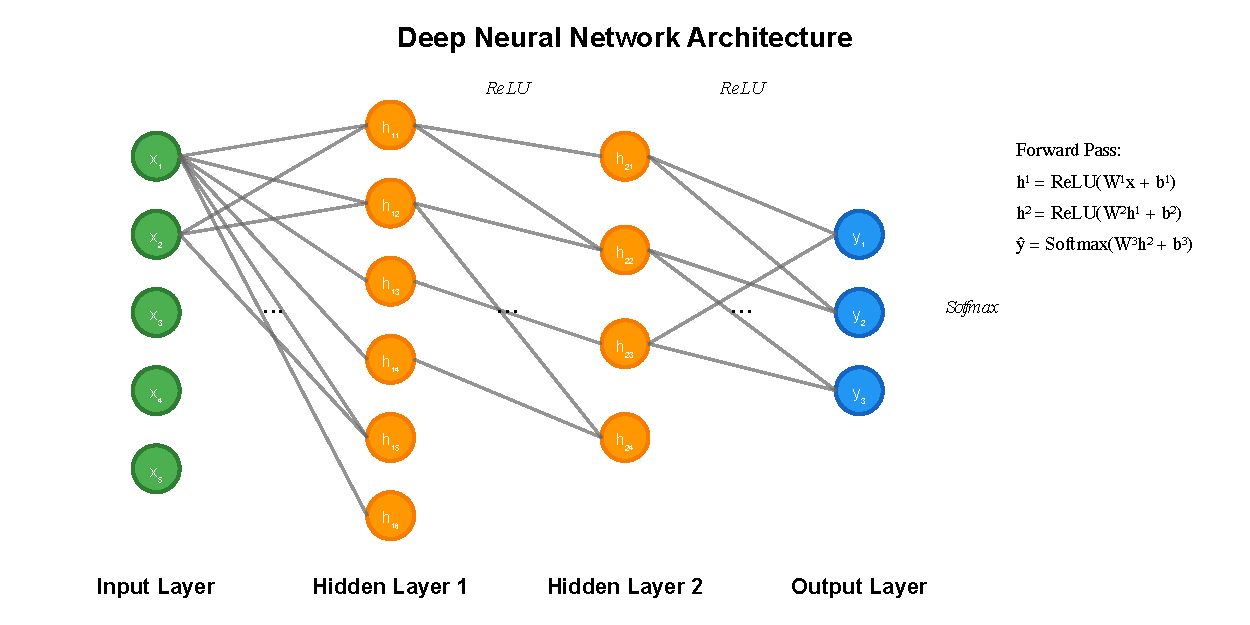
\includegraphics[keepaspectratio]{lecture_slides_files/mediabag/figures/neural_network.pdf}}

}

\caption{Neural Network Architecture}

\end{figure}%

\begin{center}\rule{0.5\linewidth}{0.5pt}\end{center}

\subsection{Deep Learning Mathematics}\label{deep-learning-mathematics}

\begin{center}\rule{0.5\linewidth}{0.5pt}\end{center}

\subsubsection{Gradient Computation via
Backpropagation}\label{gradient-computation-via-backpropagation}

The chain rule enables efficient gradient computation:

\[\frac{\partial L}{\partial W^{(l)}} = \frac{\partial L}{\partial z^{(l+1)}} \cdot \frac{\partial z^{(l+1)}}{\partial a^{(l)}} \cdot \frac{\partial a^{(l)}}{\partial W^{(l)}}\]

This slide covers gradient computation via backpropagation. Note the
mathematical expressions.

\begin{center}\rule{0.5\linewidth}{0.5pt}\end{center}

\subsubsection{Loss Function Landscape}\label{loss-function-landscape}

For classification with \(C\) classes:

\[L_{CE} = -\sum_{i=1}^{N} \sum_{c=1}^{C} y_{ic} \log(\hat{y}_{ic})\]

\begin{figure}[H]

{\centering \pandocbounded{\includegraphics[keepaspectratio]{figures/loss_function.png}}

}

\caption{Training Loss Curve}

\end{figure}%

This slide covers loss function landscape. Note the mathematical
expressions.

\begin{center}\rule{0.5\linewidth}{0.5pt}\end{center}

\subsubsection{Regularization
Techniques}\label{regularization-techniques}

\textbf{Dropout}: Randomly zero out neurons during training

\textbf{Batch Normalization}: Normalize layer inputs

\[\hat{x} = \frac{x - \mu_B}{\sqrt{\sigma_B^2 + \epsilon}}\]
\[y = \gamma \hat{x} + \beta\]

\textbf{Weight Decay}: L2 regularization on parameters

\[L_{total} = L_{data} + \lambda \sum_i w_i^2\]

\begin{figure}[H]

{\centering \pandocbounded{\includegraphics[keepaspectratio]{figures/confusion_matrix.png}}

}

\caption{Confusion Matrix}

\end{figure}%

This slide covers regularization techniques. Note the mathematical
expressions.

\begin{center}\rule{0.5\linewidth}{0.5pt}\end{center}

\subsection{Cutting-Edge Research
Directions}\label{cutting-edge-research-directions}

\begin{center}\rule{0.5\linewidth}{0.5pt}\end{center}

\subsubsection{Self-Supervised Learning}\label{self-supervised-learning}

Learning representations without labels:

\begin{itemize}
\tightlist
\item
  \textbf{Contrastive Learning}: SimCLR, MoCo, SwAV
\item
  \textbf{Masked Language Modeling}: BERT, RoBERTa
\item
  \textbf{Autoregressive Generation}: GPT, PaLM
\end{itemize}

\begin{center}\rule{0.5\linewidth}{0.5pt}\end{center}

\subsubsection{Neural Architecture Search
(NAS)}\label{neural-architecture-search-nas}

Automating architecture design:

\[\mathcal{A}^* = \arg\max_{\mathcal{A} \in \mathcal{S}} \text{Accuracy}(\mathcal{A}) - \lambda \cdot \text{Complexity}(\mathcal{A})\]

This slide covers neural architecture search (nas). Note the
mathematical expressions.

\begin{center}\rule{0.5\linewidth}{0.5pt}\end{center}

\subsubsection{Training Loop Template}\label{training-loop-template}

\begin{Shaded}
\begin{Highlighting}[]
\KeywordTok{def}\NormalTok{ train\_epoch(model, dataloader, optimizer, criterion):}
\NormalTok{    model.train()}
\NormalTok{    total\_loss }\OperatorTok{=} \DecValTok{0}
    
    \ControlFlowTok{for}\NormalTok{ batch\_idx, (data, target) }\KeywordTok{in} \BuiltInTok{enumerate}\NormalTok{(dataloader):}
\NormalTok{        optimizer.zero\_grad()}
\NormalTok{        output }\OperatorTok{=}\NormalTok{ model(data)}
\NormalTok{        loss }\OperatorTok{=}\NormalTok{ criterion(output, target)}
\NormalTok{        loss.backward()}
\NormalTok{        optimizer.step()}
\end{Highlighting}
\end{Shaded}

This slide covers training loop template. Pay attention to the code
examples.

\begin{center}\rule{0.5\linewidth}{0.5pt}\end{center}

\subsubsection{Code (continued)}\label{code-continued}

\begin{Shaded}
\begin{Highlighting}[]
        
\NormalTok{        total\_loss }\OperatorTok{+=}\NormalTok{ loss.item()}
        
        \ControlFlowTok{if}\NormalTok{ batch\_idx }\OperatorTok{\%} \DecValTok{100} \OperatorTok{==} \DecValTok{0}\NormalTok{:}
            \BuiltInTok{print}\NormalTok{(}\SpecialStringTok{f\textquotesingle{}Batch }\SpecialCharTok{\{}\NormalTok{batch\_idx}\SpecialCharTok{\}}\SpecialStringTok{, Loss: }\SpecialCharTok{\{}\NormalTok{loss}\SpecialCharTok{.}\NormalTok{item}\SpecialCharTok{:.4f\}}\SpecialStringTok{\textquotesingle{}}\NormalTok{)}
    
    \ControlFlowTok{return}\NormalTok{ total\_loss }\OperatorTok{/} \BuiltInTok{len}\NormalTok{(dataloader)}
\end{Highlighting}
\end{Shaded}

This slide covers code (continued). Pay attention to the code examples.

\begin{center}\rule{0.5\linewidth}{0.5pt}\end{center}

\subsection{Key Takeaways}\label{key-takeaways}

\begin{center}\rule{0.5\linewidth}{0.5pt}\end{center}

\subsubsection{Theoretical Insights}\label{theoretical-insights}

\begin{enumerate}
\def\labelenumi{\arabic{enumi}.}
\tightlist
\item
  \textbf{Universal Approximation}: Neural networks can approximate any
  function
\item
  \textbf{Optimization Landscape}: Non-convex but practically trainable
\item
  \textbf{Generalization}: Capacity control through regularization
\end{enumerate}

\begin{center}\rule{0.5\linewidth}{0.5pt}\end{center}

\subsubsection{Practical Guidelines}\label{practical-guidelines}

\begin{enumerate}
\def\labelenumi{\arabic{enumi}.}
\tightlist
\item
  \textbf{Start Simple}: Begin with standard architectures
\item
  \textbf{Data First}: Quality data \textgreater{} complex models
\item
  \textbf{Iterate Fast}: Rapid prototyping and experimentation
\item
  \textbf{Monitor Everything}: Loss, gradients, activations
\end{enumerate}

\begin{center}\rule{0.5\linewidth}{0.5pt}\end{center}

\subsection{References \& Further
Reading}\label{references-further-reading}

\begin{enumerate}
\def\labelenumi{\arabic{enumi}.}
\tightlist
\item
  Goodfellow, I., Bengio, Y., \& Courville, A. (2016). Deep Learning.
  MIT Press.
\item
  He, K., et al.~(2016). Deep Residual Learning for Image Recognition.
  CVPR.
\item
  Vaswani, A., et al.~(2017). Attention is All You Need. NeurIPS.
\item
  Kingma, D. P., \& Ba, J. (2015). Adam: A Method for Stochastic
  Optimization. ICLR.
\end{enumerate}

\begin{center}\rule{0.5\linewidth}{0.5pt}\end{center}

\emph{Next lecture: Advanced Topics in Generative Models}




\end{document}
